\chapter*{A Gallery of Orbits}\addcontentsline{toc}{chapter}{\protect\numberline{}A Gallery of Orbits}\markboth{A Gallery of Orbits}{A Gallery of Orbits}

\begingroup
\edef\galsavedfigure{\the\value{figure}}
\setcounter{figure}{0}
\renewcommand{\thefigure}{\arabic{figure}}
\captionsetup[figure]{name=Plate}

The pictures in this gallery are computed, not drawn.
Every point, cell and curve comes from exact integer arithmetic on the maps of \cref{chap:intro} and \cref{chap:parity} (in one plate, on the sumset of \cref{chap:cycles}), and every number quoted in a caption was produced by the script that made the picture (the files \texttt{art\_*.py} in the \texttt{scripts} directory).
We have allowed ourselves colour and a dark ground, but nothing decorative has been added: every colour encodes a computed quantity.
Throughout, $T_0$ is the standard map ($3n+1$ for odd $n$, $n/2$ for even $n$), $\sigma_\infty(n)$ is the number of steps of $T_0$ that take $n$ to $1$, its total stopping time (as in \cref{chap:intro}; \cref{chap:stochastic,chap:samplers,chap:open} count steps of $T$ instead), and $M(n)$ is the largest value on the orbit.

\begin{figure}[htb]
\centering
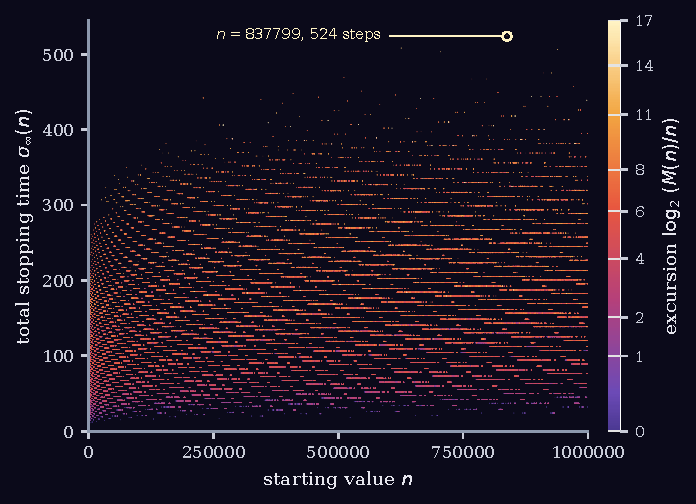
\includegraphics[width=\textwidth,height=0.78\textheight,keepaspectratio]{figures/art_g_stopping}
\caption{The total stopping time landscape. Each of the integers $2\le n\le10^6$ is
one point at height $\sigma_\infty(n)$, coloured by the excursion
$\log_2(M(n)/n)$; the longest orbit belongs to $n=837799$, with $524$ steps, and
the largest excursion to $n=159487$, which climbs to $M(n)=17\,202\,377\,752$,
a factor of about $2^{16.7}$. The horizontal streaks are runs of consecutive
integers whose orbits merge after a few steps, and the slow upward drift of the
cloud is the logarithmic growth of total stopping times discussed in
\cref{chap:intro} and \cref{chap:stochastic}.}
\label{fig:gal:stopping}
\end{figure}

\begin{figure}[p]
\centering
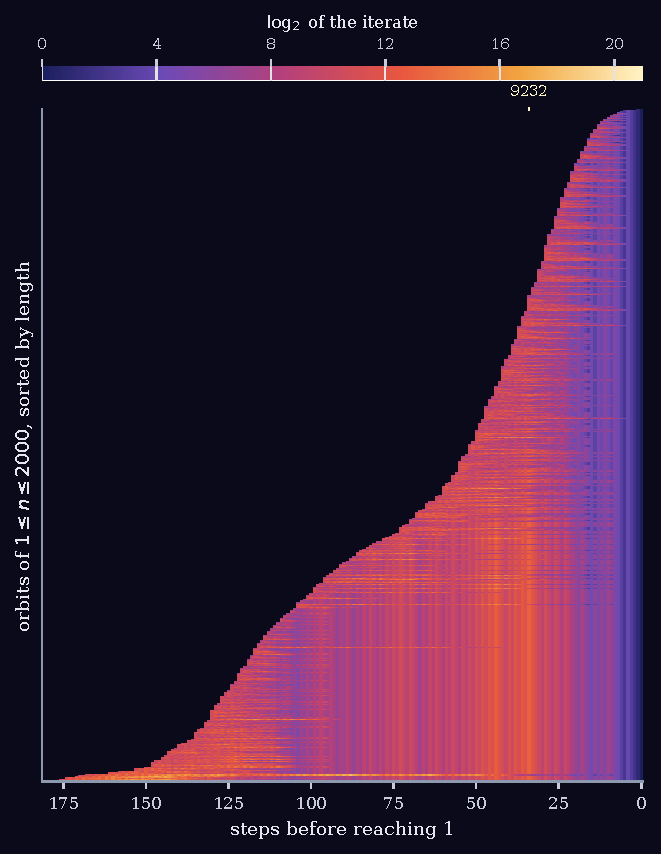
\includegraphics[width=\textwidth,height=0.78\textheight,keepaspectratio]{figures/art_g_heatmap}
\caption{The orbits of $1\le n\le2000$, one per row, written from right to left
so that every orbit ends at $1$ in the last column; colour is $\log_2$ of the
iterate, and the rows are sorted by orbit length, so the left edge is the
sorted list of total stopping times, rising to $181$ steps for $n=1161$. The bright
vertical band $34$ steps from the end is the value $9232$, through which $772$
of the $2000$ orbits pass: shared tails line up as columns, which is the
inverse tree of the next plate seen edge on.}
\label{fig:gal:heatmap}
\end{figure}

\begin{figure}[p]
\centering
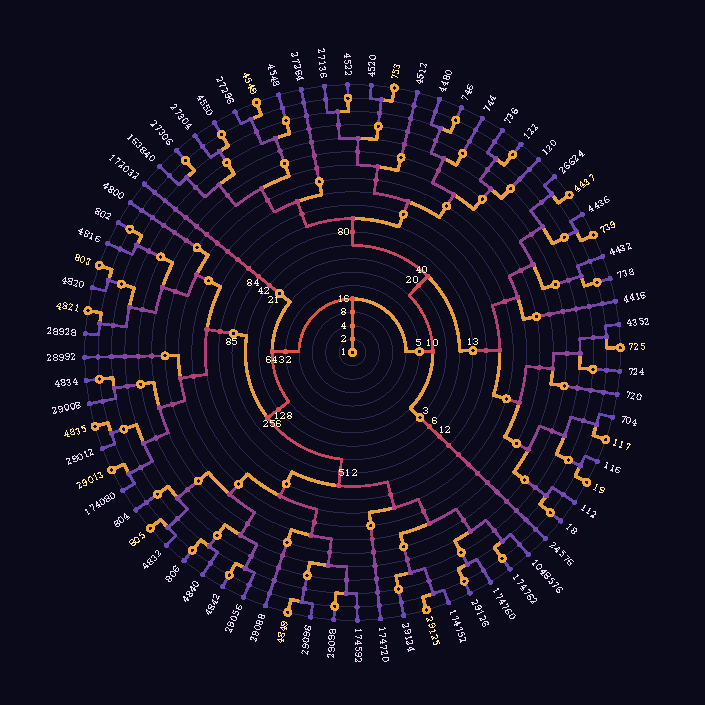
\includegraphics[width=\textwidth,height=0.78\textheight,keepaspectratio]{figures/art_g_tree}
\caption{The inverse tree of $1$ to depth $20$. The children of $m$ are $2m$ and, when $m\equiv4\pmod6$ and $m>4$, the odd number $(m-1)/3$; radius is depth, so the ring at radius $d$ holds exactly the $n$ with $\sigma_\infty(n)=d$. The tree has $342$ nodes; its $72$ leaves, the numbers with total stopping time $20$, run from $18$ to $2^{20}=1048576$, and the open circles mark the odd children, the only places where the tree branches; the branching random walk model of this tree, due to Lagarias and Weiss~\cite{lagarias1992}, is mentioned in \cref{chap:stochastic}.}
\label{fig:gal:tree}\index{Lagarias, J. C.}\index{Weiss, A.}
\end{figure}

\begin{figure}[p]
\centering
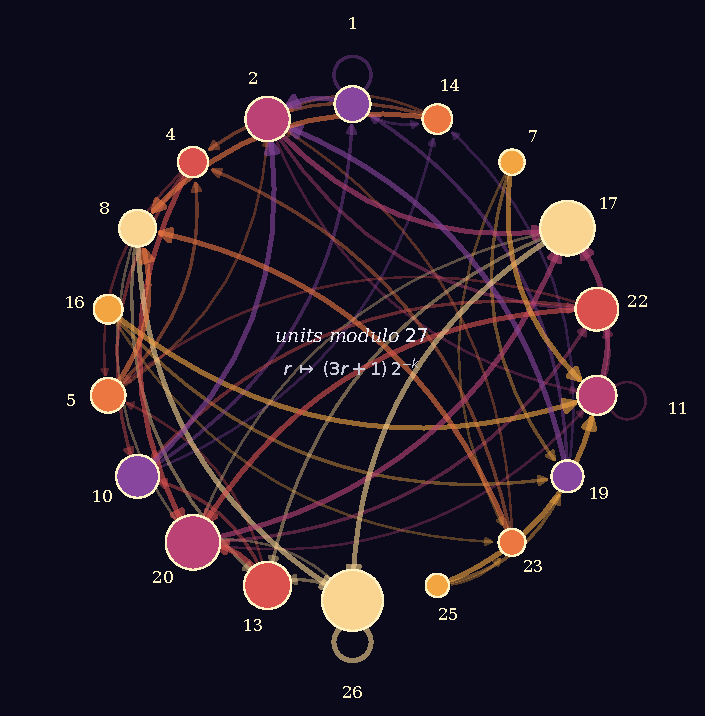
\includegraphics[width=0.94\textwidth,height=0.78\textheight,keepaspectratio]{figures/art_g_mod27}
\caption{The model chain on the $18$ units modulo $27$, in which the halving exponents are independent Geometric$(\tfrac12)$ draws: $r$ moves to $(3r+1)2^{-k}$ with probability $2^{-k}$, which for one stride from a uniformly random odd $y\equiv r$ holds exactly in the limit (\cref{chap:divergence}); with the units placed in the order $2^0,2^1,\ldots,2^{17}$, division by $2$ is one step clockwise, so the out edges of $r$ fan clockwise from $3r+1$. Edges with $k\le3$ are shown, and the three units $r$, $r+9$, $r+18$ share a shade because their common residue modulo $9$ alone determines the out edges; node area is the exact stationary law, largest at $26$ ($46570/262143\approx0.18$, with a loop of probability about $\tfrac12$) and smallest at $25$ ($1598/262143\approx0.006$), and it projects onto the law $\tfrac1{63}(8,16,11,4,2,22)$ modulo $9$.}
\label{fig:gal:mod27}
\end{figure}

\begin{figure}[p]
\centering
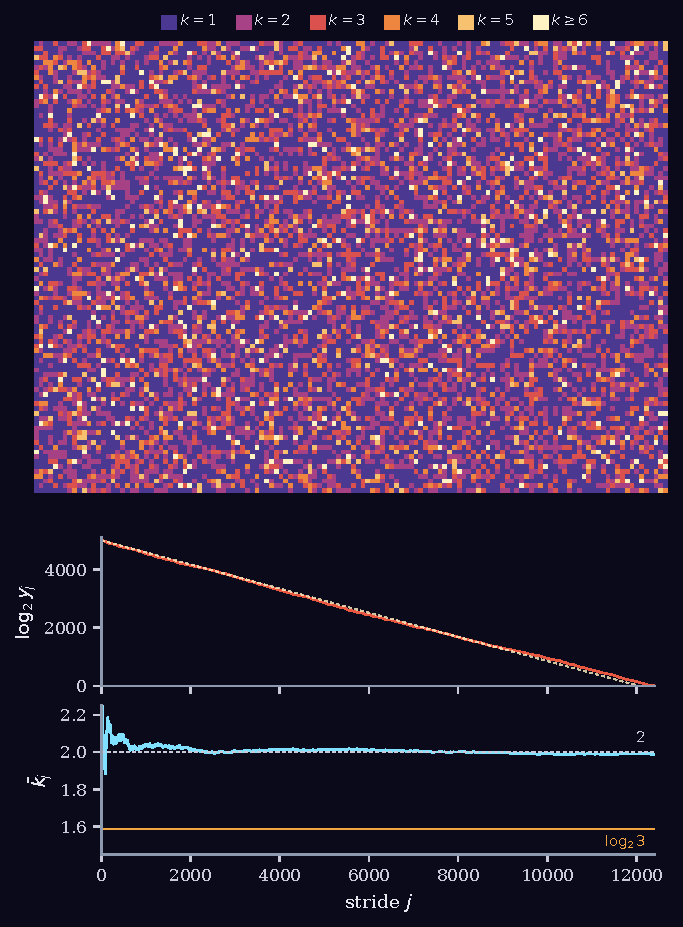
\includegraphics[width=0.9\textwidth,height=0.78\textheight,keepaspectratio]{figures/art_g_giant}
\caption{A giant orbit. Starting from $x_0=3^{3155}\approx2^{5000.56}$, the
Syracuse map takes $12408$ strides ($37075$ steps of $T_0$) to reach $1$. The
mosaic shows the exponents $k_j=\vt(3y_{j-1}+1)$ in reading order, $132$ to a
row, with frequencies $0.504$, $0.249$ and $0.128$ for $k=1,2,3$, close to the
Geometric law of \cref{chap:parity}; the descent of $\log_2y_j$
follows the drift line of slope $\log_23-2$ per stride (dashed), and the running mean
$\bar k_j$ settles near $2$, ending at $1.98799$; it lies at or below the
threshold $\log_23$ of \cref{chap:divergence} only for $j\le10$.}
\label{fig:gal:giant}
\end{figure}

\begin{figure}[p]
\centering
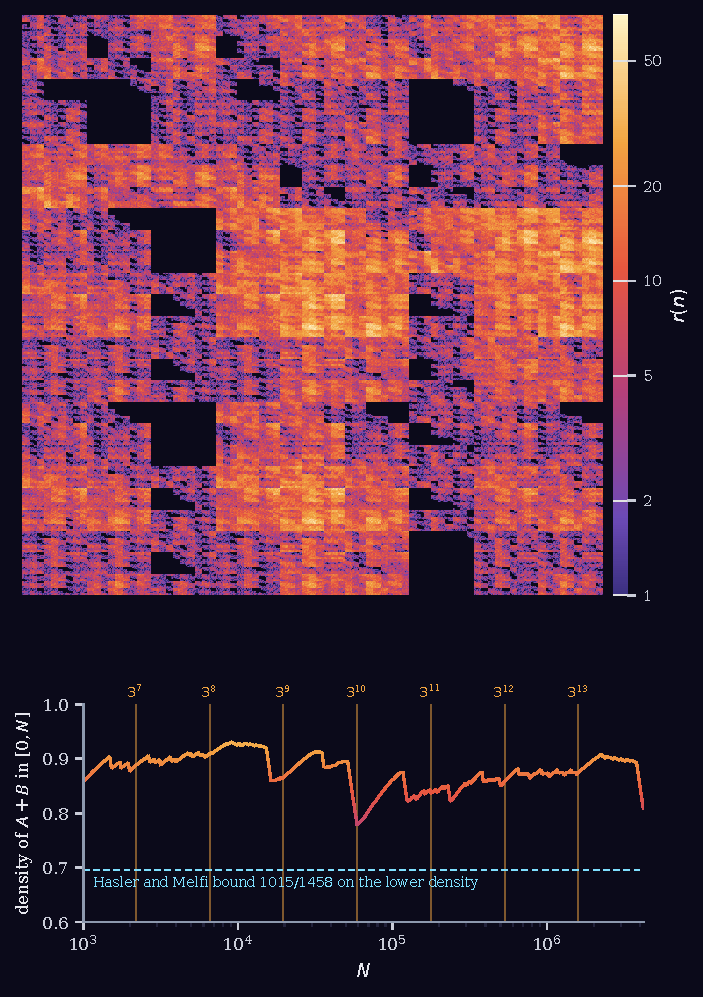
\includegraphics[width=0.9\textwidth,height=0.77\textheight,keepaspectratio]{figures/art_g_erdos}
\caption{The Erd\H{o}s $125$ sumset of \cref{chap:cycles}, with $A$ the numbers
whose base $3$ digits are $0$ or $1$ and $B$ the same in base $4$. Top: the
number $r(n)$ of representations $n=a+b$ for $n<3^{12}$, placed on a
$729\times729$ square with column and row read from the even and odd position
base $3$ digits of $n$; dark holes are gaps of $A+B$, which covers $85.83$
percent of this range, and $r(n)$ reaches $70$. Bottom: the density of $A+B$ in
$[0,N]$ for $10^3\le N\le4^{11}$, whose lowest value, $0.7785$, occurs at
$N=3^{10}-1$, well above $1015/1458\approx0.696$, the upper bound of Hasler and Melfi~\cite{haslermelfi2024} on the lower density.}
\label{fig:gal:erdos}\index{Hasler, M. F.}\index{Melfi, G.}
\end{figure}

\begin{figure}[p]
\centering
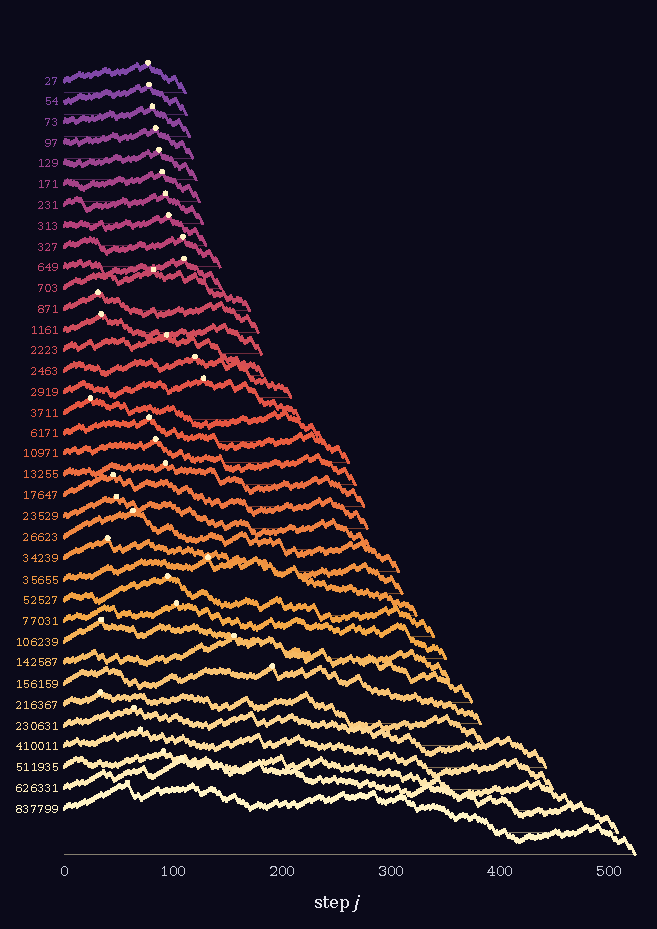
\includegraphics[width=0.92\textwidth,height=0.78\textheight,keepaspectratio]{figures/art_g_ridges}
\caption{Ridgelines of the total stopping time records. Up to $10^6$ there are $44$
integers whose total stopping time exceeds that of every smaller integer; for the
$36$ of them from $27$ ($111$ steps) to $837799$ ($524$ steps) each ridge traces
$\log_2T_0^{(j)}(n)$ until the orbit reaches $1$, with a pale dot at its
maximum. The highest summit belongs to $626331$, which climbs to
$7\,222\,283\,188$; the saw teeth are the alternation of rises by about
$\log_23$ and falls by $1$ whose net balance is the
descent problem of \cref{chap:lyapunov}.}
\label{fig:gal:ridges}
\end{figure}

\clearpage
\setcounter{figure}{\galsavedfigure}
\endgroup
